%% PNAStwoS.tex
%% Sample file to use for PNAS articles prepared in LaTeX
%% For two column PNAS articles
%% Version1: Apr 15, 2008
%% Version2: Oct 04, 2013

%% BASIC CLASS FILE
\documentclass{pnastwo}

%% ADDITIONAL OPTIONAL STYLE FILES Font specification
%\usepackage{pnastwoF}
\usepackage{graphicx,subcaption,lineno}
\usepackage{amsmath, amsthm, amsfonts, amssymb}
\usepackage{multirow,microtype}

%% OPTIONAL MACRO DEFINITIONS
\def\s{\sigma}
%%%%%%%%%%%%
%% For PNAS Only:
\url{www.pnas.org/cgi/doi/10.1073/pnas.0709640104}
\copyrightyear{2015}
\issuedate{Issue Date}
\volume{Volume}
\issuenumber{Issue Number}
%\setcounter{page}{2687} %Set page number here if desired
%%%%%%%%%%%%

\bibliographystyle{pnas}

\begin{document}

\title{Death and taxa: time-invariant differences in mammal species duration}

\author{Peter D Smits\affil{1}{University of Chicago, Chicago, Illinois,
United States of America, 60637}}

\contributor{Submitted to Proceedings of the National Academy of Sciences
of the United States of America}


%%%Newly updated.
%%% If significance statement need, then can use the below command otherwise just delete it.
\significancetext{Determining which biological traits influence differences in extinction risk is vital for understanding the differential diversification of life and for making predictions about species' vulnerability to human impacts. The durations of species in the fossil record are a rich source of information for estimating systematic differences in extinction risk. I analyzed Cenozoic North American fossil mammal durations and their relationship to multiple ecological traits, time of origination, and shared evolutionary history. I find support for generalists having lower extinction risk than specialists as a time-invariant generalization. When these results are compared to risk factors associated with living mammals, I find some incongruities which may indicate that the current biodiversity crisis is akin to the great mass extinctions in Earth's history.}

\maketitle

\begin{article}
\begin{abstract}
 Determining which biological traits influence differences in extinction risk is vital for understanding the differential diversification of life and for making predictions about species' vulnerability to anthropogenic impacts. Here I present a hierarchical Bayesian survival model of North American Cenozoic mammal species durations in relation to species-level ecological factors, time of origination, and phylogenetic relationships. I find support for the ``survival of the unspecialized'' as a time-invariant generalization of trait-based extinction risk. Furthermore, I find that phylogenetic and temporal effects are both substantial factors associated with differences in species durations. Finally, I find that the current biodiversity crisis is partially incongruous with previous patterns. This incongruity implies that pattern of mammalian background extinction for the Cenozoic is a poor predictor of the modern biodiversity crisis which is congruent how previous periods of background extinction is a poor predictor of the great mass extinctions in Earth history.
\end{abstract}

\keywords{paleobiology | macroevolution | macroecology | extinction }

%\abbreviations{}


\dropcap{W}hy extinction risk varies among species remains one of the most fundamental questions in paleobiology and conservation biology \cite{Simpson1944,VanValen1973,Raup1994,Quental2013,Wagner2014b}. To address this issue, I test for similarities in associations between extinction risk and multiple species-level traits during times of background extinction and in the modern world; which traits have time-invariant effects on species duration; and whether extinction is age-independent. I approach these questions together by using a model of species duration whose parameter estimates act as direct tests of these questions. Cenozoic mammals are an ideal focus for this study because their fossil record is well sampled and well resolved both temporally and spatially, and because individual species ecology and taxonomic position are generally understood \cite{Simpson1944,Quental2013,Alroy2009,Liow2008,Smith2004,Tomiya2013,Marcot2014}. 

Time-invariant factors are those that have a constant directional effect even if the magnitude varies. Because change in the magnitude of extinction risk is not necessarily the best indicator of a shift from background to mass extinction \cite{Wang2003}, it is better to look for changes in either the direction of selection, the loss of a selective pressure, or the appearance of novel selective pressures \cite{Jablonski1986}.

The species-level traits studied here are bioprovince occupancy, body mass, and both dietary and locomotor categories. These traits are related to aspects of a species' adaptive zone such as population density, expected range size, potential prey, and dispersal ability \cite{Smith2004,Jernvall2004}. It is expected that species with larger geographic ranges have lower extinction rates than species with smaller geographic ranges \cite{Jablonski1986,Roy2009c}; however, how traits more directly related to species--environment interactions may affect species extinction risk is more nebulous.

Body size is a complex trait related to many life history characteristics. There are three general hypotheses of how body size may effect extinction risk: 1) positive effect where an increase in body size causes an increase in extinction risk, potentially due to associated decrease in reproductive rate or similar \cite{Liow2008,Liow2009}; 2) negative effect where an increase in body size causes a decrease in extinction risk because of an expected positive relationship between body size and geographic range; and 3) no effect of body size on extinction risk \cite{Tomiya2013}. 

The strongest expectation for the effects of dietary category on extinction risk is that omnivores will have the lowest extinction risk of all species. This expectation is based on the long standing ``survival of the unspecialized'' hypothesis where more generalist species (e.g. omnivores) have greater survival than specialist species (e.g. carnivores/herbivores) \cite{Simpson1944,Liow2004a}. It has also been observed that both carnivores and herbivores have greater diversification rates than omnivores, with herbivores diversifying faster than carnivores \cite{Price2012}. How this result translates into differences in extinction risk is currently unknown \cite{Rabosky2010a}. In modern taxa, higher trophic levels (e.g. carnivores versus herbivores) have been associated with greater extinction risk, most likely because of human extermination of top predators \cite{Liow2009,Purvis2000a}. 

Similarly, there are few expectations of how locomotor category may effect extinction risk. During the Cenozoic, there was a shift at the Paleogene/Neogene boundary from predominately closed to predominately open environments \cite{Blois2009,Janis1993a}. Based on this observation, a prediction is that arboreal taxa will have the greatest extinction risk of all, with both scansorial and ground dwelling taxa having lower extinction risks. 

I use a hierarchical Bayesian survival model of species duration as predicted by the covariates of interest along with species' temporal and phylogenetic context. Species duration, in 2 My bins, was modeled as realizations from either an exponential or Weibull distribution-based hierarchical model \cite{Gelman2013d}. The exponential distribution corresponds to the Law of Constant Extinction, which states that extinction is age-independent \cite{VanValen1973}. Note that the exponential is a special case of the Weibull when its shape parameter, $\alpha$, is 1. The Weibull distribution allows for extinction to be taxon-age dependent, where values of $\alpha$ greater than 1 corresponding to increasing risk with age and values less than 1 corresponding to decreasing risk with age. Origination cohort and phylogenetic position were modeled as independent effects. Phylogenetic effect was modeled assuming species duration may have evolved via a Brownian motion-like process \cite{Lynch1991,Housworth2004}. The results from the Weibull model are detailed here because this model has a better fit to the data the exponential (Weibull WAIC 6140.37, exponential WAIC 16697.35; Fig.~\ref{fig:ppc_surv}, S1, S2).

% show results from exponential model results along side weibull results
%   make sure the signs are the same for exponential and weibull?
%     then I can show estimates together with double histograms?
%     will really help explain the actual results
%   do as two histograms in the same panel for the posterior predictive checks!
%     probably just in supplement
%   results are consistent with which hypotheses?

\section{Results}
A summary of the posterior distributions for the most relevant parameter estimates is presented in Table \ref{tab:post_sum}. All posterior inference is based on these estimates. For the results from the posterior predictive checks and discussion of the estimation of $\alpha$, please see the accompanying Supplemental information. Additionally, See the Supplemental information for discussion surrounding use of Paleobiology Database and accompanying data quality concerns.

Species with greater bioprovince occupancy are found to be associated with lower extinction risk than taxa with smaller bioprovince occupancy (\(\beta_{occupancy} \text{mean} = -0.53\), std \(= 0.08\)). This is consistent with previous findings. Body size has nearly zero association with expected duration (\(\beta_{size} \text{mean} = -0.05\), std \(= 0.05\)), a similar result to some previous studies \cite{Tomiya2013}. However, previous studies were performed at the generic level and were unable to determine how body size may effect species-level extinction, as the effect of either extinction or speciation cannot be distinguished \cite{Liow2008,Tomiya2013}.

Some clear patterns emerge from the pairwise differences in effect of each dietary category on expected duration (Fig.~\ref{fig:trait_est}). Consistent with expectations from the ``survival of the unspecialized'' hypothesis \cite{Liow2004a,Simpson1944}, omnivory appears to be associated with the lowest expected extinction risk. Carnivory is associated a greater expected duration than either herbivory or insectivory, but a greater expected extinction risk than omnivory. Finally, herbivory and insectivory have approximately equal effects on expected duration. Given previous results, these results imply that carnivores have a greater origination rate than omnivores \cite{Price2012}. These results also imply that herbivores, which have the greatest extinction risk, must also have a very high origination rate in order to have the greatest diversification rate among these three categories \cite{Price2012}. 

For locomotor category, both scansoriality and ground dwelling life habitat are associated with a greater expected duration than arboreality (Fig.~\ref{fig:trait_est}). Scansorial and ground dwelling life habits also have approximately equal expected effects on extinction risk.  This is consistent with the expectation that arboreality will confer greater extinction risk due to the loss of associated environment with the shift from open to closed habitat at the Paleogene/Neogene boundary \cite{Blois2009}. However, there are two possible processes which could lead to the observed pattern: arboreality confers an intrinsic difference in extinction risk or it might not be that arboreal taxa have an intrinsically higher risk but were instead ``hit harder'' by the environmental shift than other taxa. This analysis cannot distinguish between these two processes. Note that in the case of European Cenozoic mammals, this period corresponds to the Vallesian which involved a dramatic shift in species demography \cite{Agusti2013,Moya-Sola2005}.

Of the three sources of variance present in the model, individual species variance accounts for approximately 80\% of the observed, unmodeled variance (Fig.~\ref{fig:vpc}). Note that the individual variance was approximated using an simulation approach \cite{Goldstein2002} because the Weibull distribution does not have a variance term. Both cohort and phylogenetic effects account for the other 20\% of the observed variance. This result means that extinction risk has both temporal and phylogenetic aspects, as both contribute greater than 0\% of the observed variability in the data \cite{Housworth2004}. This result lends credence to the hypothesis that extinction rate is heritable \cite{Rabosky2009e}.

% decrease in extinction risk with time is known previous result
% plot S(t) for each cohort with posterior predictive checks as panels?
%   this is probably very useful way of depicting variance in cohort survival functions
% two part figure 
%   Exponential and Weibull fit to S(t)
%   facet grid with each cohort S(t)
%     show Exponential and Weibull fits per cohort, two overlaping colors
The estimates for the individual cohort effects show a weak pattern of greater extinction risk in older Cenozoic cohorts compared to younger cohorts (Fig.~\ref{fig:eff_cohort}). This potential slowdown in extinction risk is consistent with previous analyses of marine invertebrates \cite{Raup1982a,Foote2003} and mammals \cite{Alroy2010c,Alroy2000g}. There are two prevailing hypotheses as to the cause of this slowdown: 1) extinction risk is constant within, but varies between, clades so over time clades with low extinction rates increases in proportion of total diversity thus bringing down expected extinction risk; or 2) over time taxa increase in mean fitness and thus decrease in expected extinction risk \cite{Raup1982a}. The observed decrease in extinction risk with age, along with the variance partitioning results (Fig.~\ref{fig:vpc}) are consistent with both of these hypotheses with neither being more ``important'' than the other. 

Interestingly, the shift from older cohorts with a higher extinction risk to younger cohorts with lower extinction risk is approximately at the Paleogene--Neogene boundary. Given the association with arboreality (a heritable trait) and increased extinction risk (Fig.~\ref{fig:trait_est}), the decrease in expected extinction risk over time might relate to the preferential loss of arboreal taxa over the Cenozoic. However, because the model used here does not allow for time-varying effects, I cannot identify whether this boundary is associated with a shift in the direction or magnitude of the expected effect of arboreality on extinction risk.

\section{Discussion}
My results indicate that overall, for Cenozoic mammals, generalists are expected to have a lower extinction risk than specialists. This implies that the diversification of specialized taxa was not driven by biased extinction. Instead, an increase in diversity would have required either a driven trend away from generality \cite{McShea1994a} or an increase in speciation rate relative to extinction rate \cite{Stanley1975}. This requires that specialist traits should somehow increase or be associated with increases in speciation rate, perhaps via niche partitioning or changes in habitat heterogeneity. For example non-omnivores may more finely divide available prey items or arboreal taxa may increase in both extinction and speciation rates via increases in habitat heterogeneity. Possible evident to support this hypothesis would be to demonstrate that differences in speciation rate are different than those demonstrated here for extinction risk.

When these results are compared to factors contributing to increased extinction risk in extant mammals, there are some incongruencies. As expected, large range size is consistently associated with lower extinction risk in the modern world \cite{Liow2009,Purvis2000a,Fritz2009,Fritz2010b}. While my analysis found body size to have almost no time-invariant effect on extinction risk, in extant mammals this is not necessarily the case as increased body size is associated with increased extinction risk \cite{Liow2009,Purvis2000a}. However, this pattern is partially clade dependent \cite{Fritz2009}. As stated earlier, higher trophic levels have been found to be associated with greater extinction risk in extant mammals \cite{Liow2009,Purvis2000a}. In contrast, I found that omnivores and carnivores have a lower expected extinction risk than either insectivores or herbivores (Fig.~\ref{fig:trait_est}). Finally, phylogeny has been found to be a good predictor of differences in extinction risk in extant mammals as certain clades are at much higher risks than others \cite{Fritz2010b}. This effect seems much greater in the Recent than for the whole Cenozoic, implying that current extinction risk is more phylogenetically concentrated than during times of background extinction levels during the Cenozoic.

Whether these incongruities are within the standard range of time-variant effects is unknown, though my comparisons do imply that current processes are different from those studied here. These inconsistencies imply that the fossil record may not provide a guide for conservation biology. However, this is not a model of what makes taxa vulnerable during mass extinctions and that may account for these incongruities, assuming mass extinctions are qualitatively different than background extinction \cite{Jablonski1986}. These results would also be inapplicable if the current biodiversity crisis is qualitatively different from either background or mass extinction as preserved in the fossil record.

By modeling how different ecologies and historical factors effect a species' expected extinction risk, it is possible to better understand what processes may have driven the resulting pattern of selection (i.e. diversity). This analysis finds support for the ``survival of the unspecialized'' hypothesis \cite{Simpson1944,Liow2004a} as a time-invariant generalization about extinction risk. I also find that there are substantial effects of both cohort and phylogeny on extinction risk, which supports the idea that the decrease in extinction risk \cite{Raup1982a} over time has both temporal and phylogenetic components. Additionally, I found evidence of increasing extinction risk with species age, the cause of which is unknown. These results show that, like prior mass extinction events in the fossil record, the current biodiversity crisis is qualitatively different from the previous period of background extinction in the fossil record \cite{Jablonski1986}.


\begin{materials}
\section{Species occurrence and covariate information}
Fossil occurrence information was downloaded from the Paleobiology Database (PBDB; http://paleodb.org/). Occurrence, taxonomic, stratigraphic, and biological information was downloaded for all North American mammals. This data set was filtered so that only occurrences identified to the species-level, excluding all ``sp.''-s. All aquatic and volant taxa were also excluded. Additionally, all occurrences without latitude and longitude information were excluded from the sample.

Species dietary and locomotor category assignments were done using the assignments in the PBDB, which were reassigned into coarser categories (Supplementary Table S1). This was done to improve interpretability, increase sample size per category, and make results comparable to previous studies \cite{Jernvall2004,Price2012}.

All individual fossil occurrences were assigned to 2 My bins ranging through the entire Cenozoic. Taxon duration was measured as the number of 2 My bins from the first occurrence to the last occurrence, inclusive. This bin size was chosen because it approximately reflects the resolution of the North American Cenozoic mammal fossil record \cite{Alroy2009,Alroy2000g,Marcot2014}. Species originating in the youngest cohort, 0-2 My, were excluded from analysis because every species duration would be both left and right censored, which is illogical.

Species body size estimates in grams were sourced from a large selection of primary literature and database compilations. Databases used include the PBDB, PanTHERIA \cite{Jones2009c}, and the Neogene Old World Mammal database (NOW; http://www.helsinki.fi/science/now/). Major sources of additional compiled body size estimates include \cite{Tomiya2013,Brook2004a,Freudenthal2013,McKenna2011,Raia2012f,Smith2004c}. These were then supplemented with an additional literature search to try and fill in the remaining gaps. In many cases, species body mass was estimated using various published regression equations based on tooth or skull measurements (Supplementary Table S2). If multiple specimens were measured, I used the mean of specimen measures as the species mean. See Supplemental Dataset 1 for a complete list of mass estimates and sources.

\subsection{Biogeographic network}
Species geographic extent was measured as the mean of the relative number of bioprovinces occupied by a species for each 2 My bin the species was present. Bioprovinces were identified using a network-theoretic approach that has previously been applied to paleontological data \cite{Sidor2013,Vilhena2013}. This approach relies on defining a biogeographic bipartite network of taxa and localities. In this study, taxa were defined as species and localities were grid cells from a regular lattice on a global equal-area cylinder map projection. The regular lattice was defined as a 70 x 34 global grid where each cell corresponds to approximately 250000 km\(^{2}\). An advantage of this approach is that this approach reduces to occupancy when all localities are independent and to a single bioprovince when all localities are identical.

A biogeographic network was constructed for each of the 2 My bins used in this study. Emergent bioprovinces were then identified using the map equation \cite{Rosvall2008,Rosvall2009a} as has been done before \cite{Sidor2013,Vilhena2013b,Vilhena2013}. These bioprovinces correspond to taxa and localities that are more interconnected with each other than with other nodes.

The map projection and regular lattice were made using shape files from http://www.naturalearthdata.com/ and the \texttt{raster} package for R \cite{raster}. Bioprovince identification was done using the map equation as implemented in the \texttt{igraph} package for R \cite{csardi2006igraph}.


\subsection{Supertree}

As there is no single, combined formal phylogenetic hypothesis of all Cenozoic fossils mammals from North America, it was necessary to construct a semi-formal supertree. This was done by combining taxonomic information for all the observed species and a few published phylogenies using matrix representation parsimony \cite{Bininda-Emonds2007}. For further explination of the methodology used to construct this supertree, please see the Supplementary information.


\section{Survival model}
Presented here is the model development process used to formulate the two survival models used in this study. First, define \(y\) as a vector of length \(n\) where the \(i\)th element is the duration of species \(i\), where \(i = 1,\cdots,n\).

The simplest survival model where durations are assumed to follow an exponential distribution with a single ``rate'' or inverse-scale parameter \(\lambda\) \cite{Klein2003}. This is written
\begin{align}
  p(y | \lambda) &= \lambda \exp(-\lambda y) \nonumber \\
  y &\sim \mathrm{Exp}(\lambda).
  \label{eq:exp}
\end{align}
The exponential distribution corresponds to situations where extinction risk is independent of age. To understand this, we need to define two functions: the survival function \(S(t)\) and the hazard function \(h(t)\). \(S(t)\) is the probability that a species having existed for \(t\) 2 My bins will not have gone extinct while \(h(t)\) corresponds to the instantaneous extinction rate for some taxon age \(t\) \cite{Klein2003}. For an exponential model, \(S(t)\) is 
\begin{equation}
  S(t) = \exp(-\lambda t)
  \label{eq:exp_surv}
\end{equation}
and \(h(t)\) is defined
\begin{equation}
  h(t) = \lambda
  \label{eq:exp_haz}
\end{equation}
The choice of the exponential distribution corresponds directly to the Law of Constant Extinction \cite{VanValen1973} as the right side of Eq.~\ref{eq:exp_haz} does not depend on species age \(t\). 

The current sampling statement (Eq.~\ref{eq:exp}) assumes that all species share the same rate parameter with no variation. To allow for variation in \(\lambda\) associated with relevant covariate information like species body size, \(\lambda\) is reparameterized as \(\lambda_{i} = \exp(\sum \beta^{T}\mathbf{X}_{i})\) with \(i\) indexing a given observation and its covariates, \(\beta\) is a vector of regression coefficients, and \(\mathbf{X}\) is a matrix of covariates. This is a standard regression approach, where one column of \(\mathbf{X}\) is all 1-s and its corresponding \(\beta\) coefficient is the intercept. 

To relax the assumption of age-independent extinction of the Law of Constant Extinction, the Weibull distribution is substituted for the exponential \cite{Klein2003}. The Weibull distribution has a shape parameter \(\alpha\) and scale parameter \(\sigma\). Conceptually, \(\sigma\) is the inverse of \(\lambda\). \(\alpha\) modifies the impact of taxon age on extinction risk. When \(\alpha > 1\) then \(h(t)\) is a monotonically increasing function, but when \(\alpha < 1\) then \(h(t)\) is a monotonically decreasing function. When \(\alpha = 1\) then the Weibull distribution is equivalent to the exponential.

The Weibull distribution and sampling statement were defined
\begin{align}
  p(y | \alpha, \sigma) &= \frac{\alpha}{\sigma} \left(\frac{y}{\sigma}\right)^{\alpha - 1} \exp\left(-\left(\frac{y}{\sigma}\right)^{\alpha}\right) \nonumber \\
  y &\sim \mathrm{Weibull}(\alpha, \sigma).
  \label{eq:weibull}
\end{align}
The corresponding \(S(t)\) and \(h(t)\) functions are defined
\begin{align}
  S(t) &= \exp\left(-\left(\frac{t}{\sigma}\right)^{\alpha}\right) \label{eq:wei_surv} \\
  h(t) &= \frac{\alpha}{\sigma}\left(\frac{t}{\sigma}\right)^{\alpha - 1} \label{eq:wei_haz}.
\end{align}

To allow for \(\sigma\) to vary with a given observation's covariate information it is reparameterized in a similar fashion to \(\lambda\) with a few key differences. Because \(\sigma = 1/\lambda\) in order to preserve the interpretation of \(\beta\), while taking \(\alpha\) into account, \(\sigma\) is reparameterized as
\begin{equation}
  \sigma_{i} = \exp\left(\frac{-(\beta)}{\alpha}\right).
  \label{eq:reg}
\end{equation}

Given the above, the survival model was then fit in a Bayesian context using both the exponential and Weibull based models. The Weibull's \(\alpha\) parameter was assumed constant across species, which is standard practice in survival analysis \cite{Klein2003}. \(\alpha\) was given a weakly informative half-Cauchy (C\(^{+}\)) prior. \(\sigma\) was reparameterized as an exponentiated regression model (Eq.~\ref{eq:reg}). This was further expanded (Eq.~\ref{eq:wei_reg_ext}) to allow for two hierarchical factors as discussed below. This is written
\begin{equation}
  \sigma_{i} = \exp\left(\frac{-(h_{i} + \eta_{j[i]} + \sum \beta^{T} \mathbf{X}_{i})}{\alpha}\right)
  \label{eq:wei_reg_ext}
\end{equation}
where equivalent statement for the exponential distribution is defined
\begin{equation}
  \lambda_{i} = \exp\left(h_{i} + \eta_{j[i]} + \sum \beta^{T} \mathbf{X}_{i})\right).
  \label{eq:exp_reg_ext}
\end{equation}

\(\mathbf{X}\) is an \(n \times K\) matrix of species-level covariates. Three of the covariates of interest are the logit of mean relative occupancy, and the logarithm of body size (g). The discrete covariate index variables of dietary and locomotor category were transformed into \(n \times (k - 1)\) matrices where each column is an indicator variable (0/1) for that species's category, \(k\) being the number of categories of the index variable (3 and 4, respectively). Only \(k - 1\) indicator variables are necessary as the intercept takes on the remaining value. For example, the difference in effect of arboreality versus scansoriality on extinction risk, given that arboreality is the reference category, is the coefficient for the scansorial indicator variable as that is the difference between between the effect of arboreality (the intercept) and scansoriality (the intercept + scansorial effect; Fig. \ref{fig:trait_est}). 

Finally, a vector of 1-s was included in the matrix \(\mathbf{X}\) whose corresponding \(\beta\) coefficient is the intercept, making \(K\) equal eight.

\(\beta\) is the vector of regression coefficients. The intercept term was given a weak normal prior, \(\beta_{0} \sim \mathcal{N}(0, 10)\) while all of these other coefficients were slightly more informative priors, e.g. \(\beta_{mass} \sim \mathcal{N}(0, 5)\). These priors were chosen because it is expected that the effect size of each variable on duration will be small, as is generally the case with binary covariates \cite{Gelman2007}. %In all cases, posterior inference was not effected by changes to this choice of prior. Do I have proof?

Regression coefficients are not directly comparable without first standardizing the input variables to have equal standard deviations. This is accomplished by subtracting the mean of the covariate from all values and then dividing by the standard deviation, resulting in a variable with mean of zero and a standard deviation of one. This linear transform greatly improves the interpretability of the coefficients as expected change in mean duration given a difference of one standard deviation in the covariate \cite{Schielzeth2010}. Additionally, this makes the intercept directly interpretable as the estimate of mean (transformed) \(\sigma\) (Eq.~\ref{eq:reg}). However, because the expected standard deviation for a random binary variable is 0.5, in order to make comparisons between the binary and continuous variables, the continuous inputs were divided by twice their standard deviation \cite{Gelman2008}. 

Origination cohort is defined as the group of species which all originated during the same 2 My temporal bin. Because the most recent temporal bin, 0-2 My, was excluded, there are 32 total cohorts. The effect of origination cohort \(j\) was modeled with each group being a sample from a common cohort effect, \(\eta\), which was considered normally distributed with mean 0, and standard deviation \(\sigma_{c}\). The value of \(\sigma_{c}\) was then estimated from the data itself, corresponding to the amount of pooling in the individual estimates of \(\eta_{j}\). This approach is a conceptual and statistical unification between dynamic and cohort survival analysis in paleontology \cite{Foote1988,Raup1978,Raup1975,VanValen1979,Baumiller1993}, with \(\sigma_{c}\) acting as a measure of compromise between these two end members. The choice of the half-Cauchy prior for \(\sigma_{c}\) follows \cite{Gelman2006a}.
\begin{align*}
  \eta_{j} &\sim \mathcal{N}(0, \sigma_{c}) \\
  \sigma_{c} &\sim \mathrm{C}^{+}(0, 2.5)
\end{align*}

The impact of shared evolutionary history, or phylogeny, was modeling as an individual effect where each observation, \(i\), is modeled as a multivariate normal, \(h\), where the covariance matrix \(\Sigma\) is known up to a constant, \(\sigma_{p}^{2}\) \cite{Lynch1991,Housworth2004}. This is written
\begin{align*}
  h &\sim \mathrm{MVN}(0, \mathbf{\Sigma}) \\
  \mathbf{\Sigma} &= \sigma_{p}^{2} \mathbf{V}_{phy} \\
  \sigma_{p} &\sim \mathrm{C}^{+}(0, 2.5).
\end{align*}

\(\mathbf{V}_{phy}\) is the phylogenetic covariance matrix defined as an \(n \times n\) matrix where the diagonal elements are the distance from root to tip, in branch length, for each observation and the off-diagonal elements are the amount of shared history, measured in branch length, between observations \(i\) and \(j\). \(\sigma_{p}\) was given a weakly informative half-Cauchy hyperprior. Note that because the phylogeny used here is primarily based on taxonomy, estimates of \(\sigma_{p}\) represent minimum estimates \cite{Lynch1991,Housworth2004}. Improved phylogenetic estimates of all fossil Cenozoic mammals would greatly improve this estimate.

An important part of survival analysis is the inclusion of censored observations where the failure time has not been observed \cite{Ibrahim2001,Klein2003}. The most common censored observation is right censored, where the point of extinction had not yet been observed in the period of study, such as taxa that are still present in the most recent time bin (0-2 My). Left censored observations, on the other hand, correspond to observations that went extinct any time between 0 and some known point. To account for this uncertainty, the probability of a left censored observation is found by integrating over all possible durations between 0 and 1 time bin. For an explanation of how censored observations are included in the sampling statement, please see the Supplementary information.


\section{Estimation}
Parameter posteriors were approximated using a Markov-chain Monte Carlo (MCMC) routine implemented in the Stan programming language \cite{2014stan}. Stan implements a Hamiltonian Monte Carlo using a No-U-Turn sampler \cite{Hoffman-Gelman:2011}. Posterior approximation was done using four parallel MCMC chains run for 30000 steps, thinned to every thirtieth sample, split evenly between warm-up and sampling. Convergence was evaluated using the scale reduction factor, \(\hat{R}\). Values of \(\hat{R}\) close to 1, or less than or equal to 1.1, indicate approximate convergence. Convergence means that the chains are approximately stationary and the samples are well mixed \cite{Gelman2013d}.


\section{Posterior evaluation}
The most basic assessment of model fit is that simulated data generated given the model should be similar to the observed. This is the idea behind posterior predictive checks. Using the covariates from each of the observed durations, and randomly drawn parameter estimates from their marginal posteriors, a simulated data set \(y^{rep}\) was generated. This process was repeated 1000 times and the distribution of \(y^{rep}\) was compared with the observed \cite{Gelman2013d}. For results from the posterior predictive tests used in this study, please see the Supplementary information.

The exponential and Weibull models were compared for out-of-sample predictive accuracy using the widely-applicable information criterion (WAIC) \cite{Watanabe2010a}. Because the Weibull model reduces to the exponential model when \(\alpha = 0\), our interest is not in choosing between these models. Instead comparison of WAIC values is useful for better understanding the effect of model complexity on out-of-sample predictive accuracy. An explanation of how WAIC is calculated is presented in the Supplementary information following the ``WAIC 2'' formulation recommended by \cite{Gelman2013d}.

There are three different variance components in this model: sample \(\sigma_{y}^{2}\), cohort \(\sigma_{c}^{2}\), and phylogenetic \(\sigma_{p}^{2}\). The sample variance, \(\sigma_{y}^{2}\), is similar to the residual variance from a normal linear regression. Partitioning the variance between these sources allows the relative amount of unexplained variance of the sample to be compared. However, the Weibull based model used here (Eq.~\ref{eq:weibull}) does not include an estimate of the sample variance, \(\sigma_{y}^{2}\). Partitioning the variance between these three components was approximated via a simulation approach modified from \cite{Goldstein2002}. For explanation of this method, please see Supplementary information.

I used variance partitioning coefficients (VPC) to estimate the relative importance of the different variance components \cite{Gelman2007}. Phylogenetic heritability, \(h_{p}^{2}\) \cite{Lynch1991,Housworth2004}, is identical to the VPC of the phylogenetic effect. Additionally, because phylogenetic effect was estimated using a principally taxonomy based tree the estimates derived here can be considered minimum estimates of the phylogenetic effect.
\end{materials}

\begin{acknowledgments}
P.D.S would like to thank M. Foote, K. Angielczyk, R. Ree, P.D. Polly for discussion; N. Pierrehumbert, E. Sander, L. Southcott for draft comments; and J. Alroy and the Fossilworks/Paleobiology Database for data accumulation, management, and availability. This is Paleobiology Database publication number XXX.
\end{acknowledgments}

\bibliography{newbib,packages}

\end{article}

\begin{figure}[ht]
  \centering
  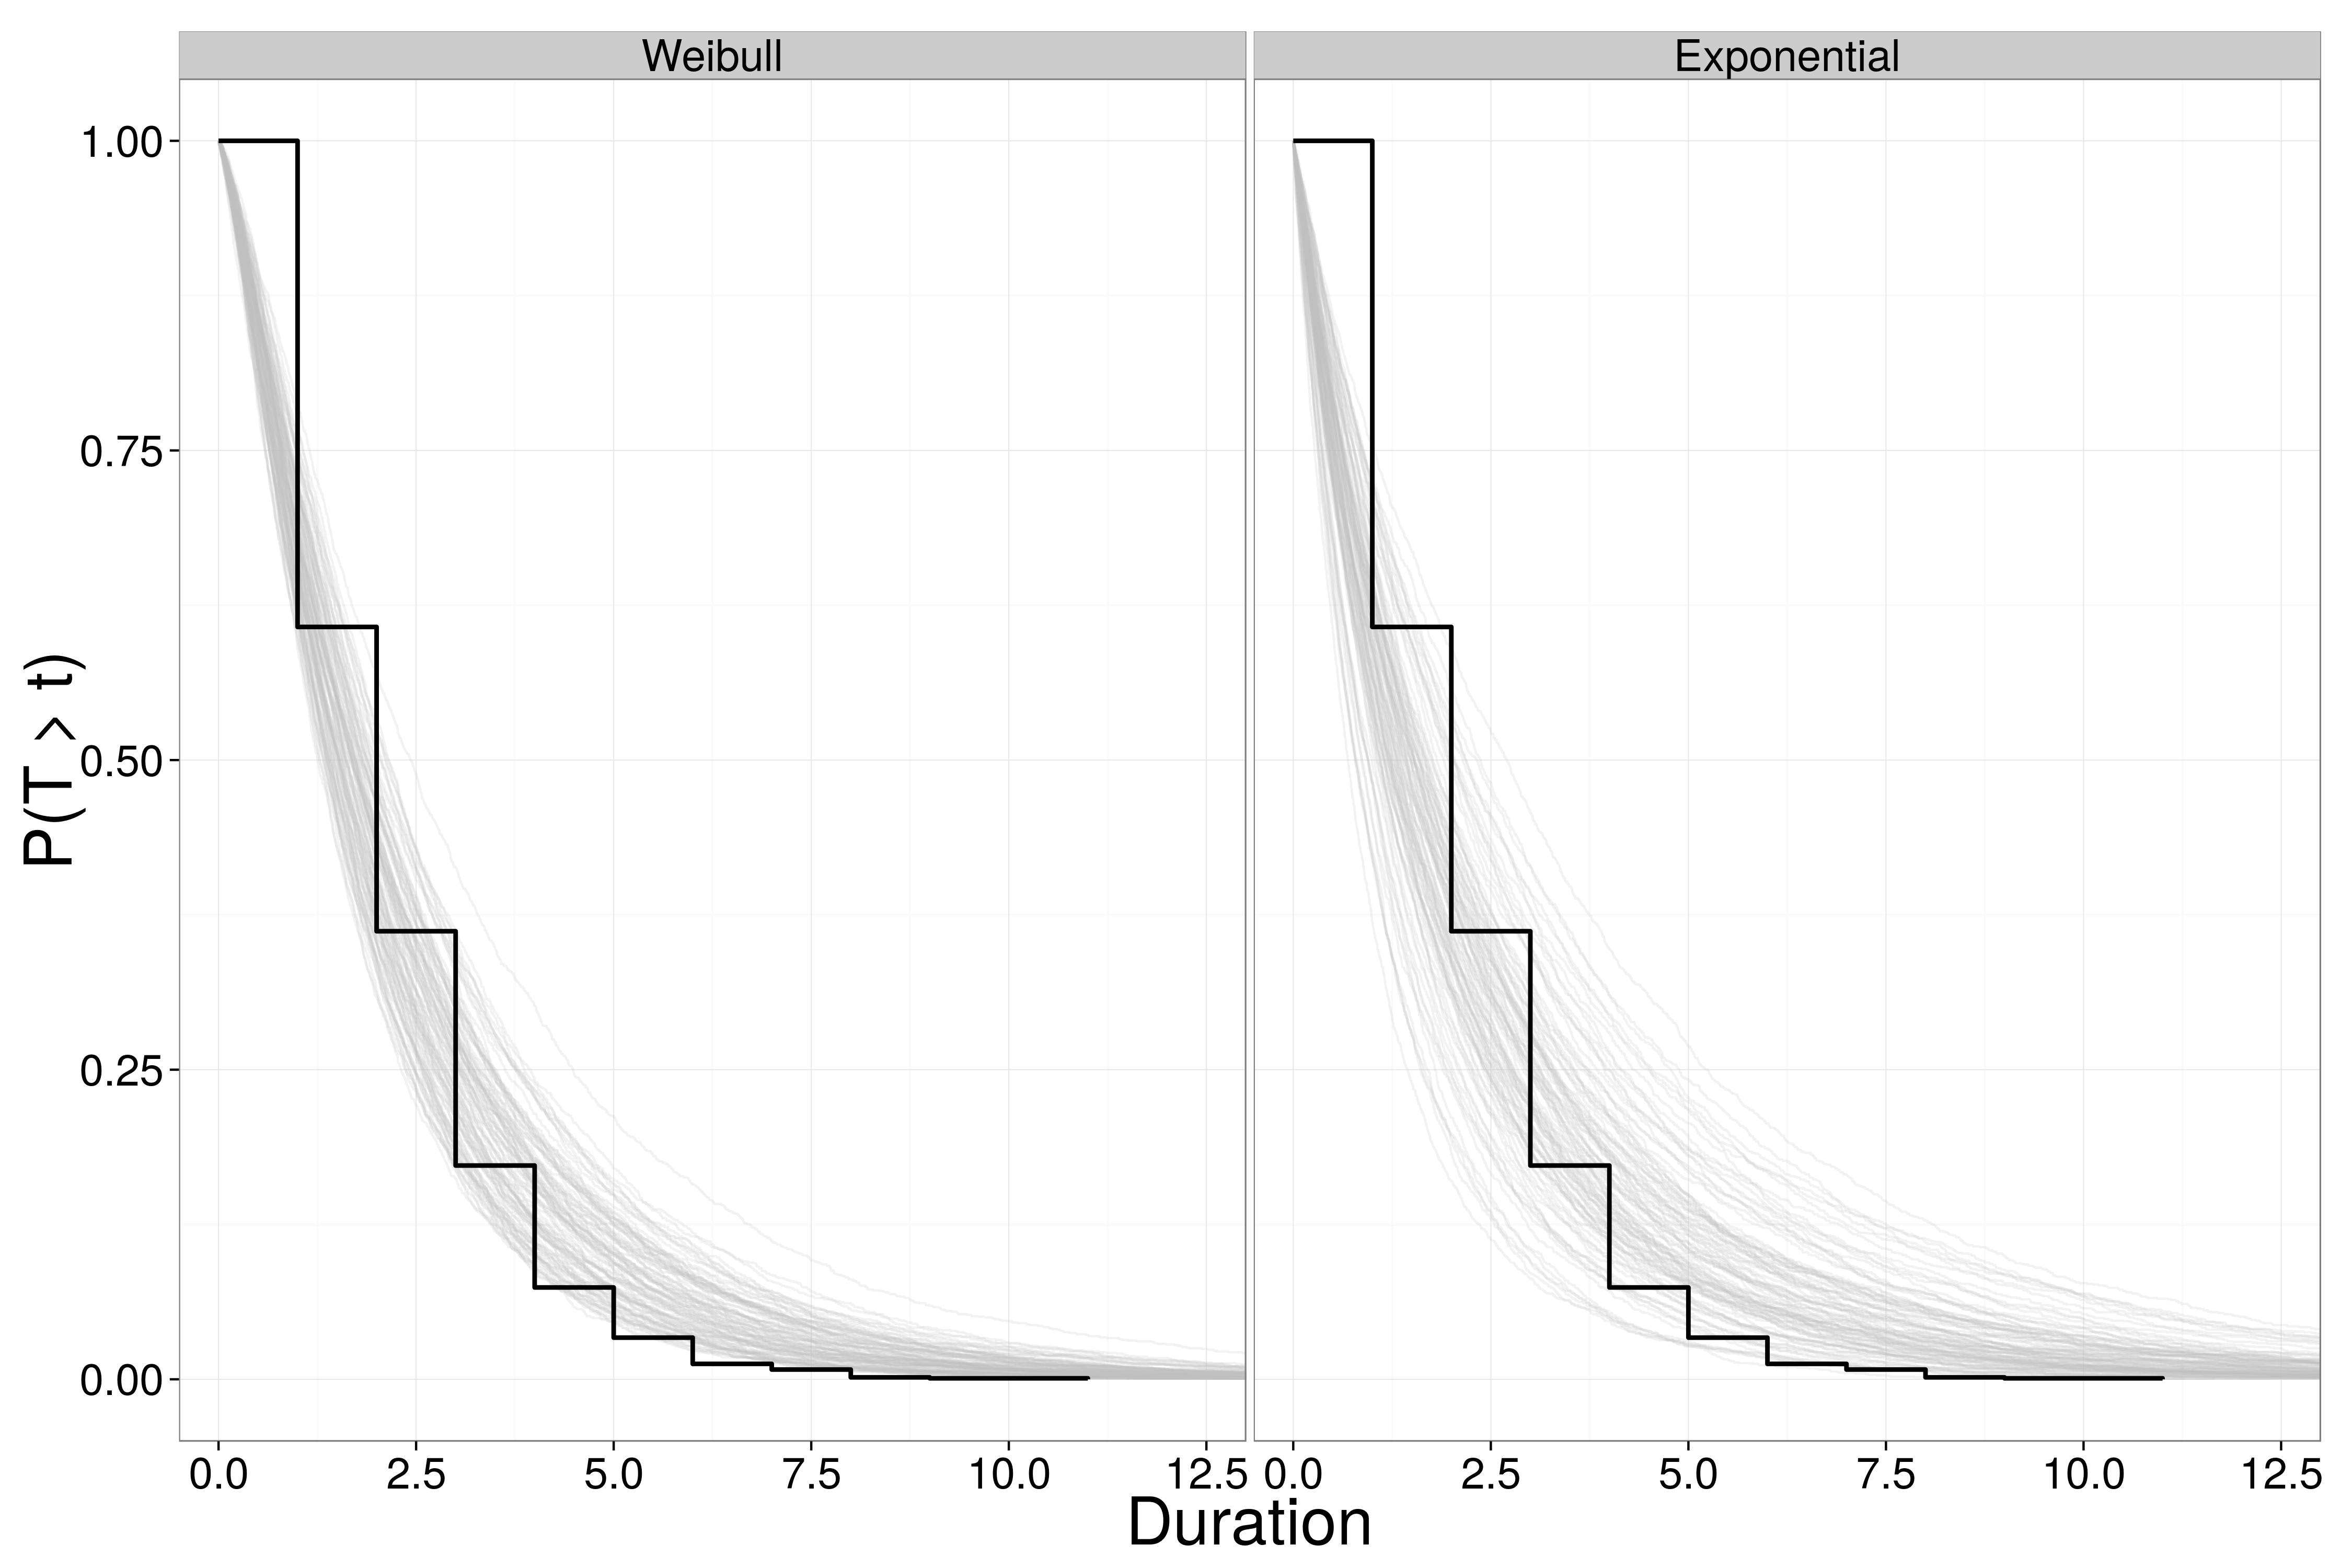
\includegraphics{figure/survival_function}
  \caption{Comparison of estimates of the empirical survival function (black) and survival functions from 1000 simulated data sets using the fitted model (dark grey). The survival function is the probability that a species with duration \(t\) will not have gone extinct. Simulated data sets were generated by drawing parameter values randomly from their estimated posteriors and using the observed covariate information to estimate durations for all the observed species. On the left are the results from the exponential survival model, while on the right are the results the Weibull model.}
  \label{fig:ppc_surv}
\end{figure}

\begin{figure}[ht]
  \centering
  \begin{subfigure}[b]{0.4\textwidth}
    \caption{}
    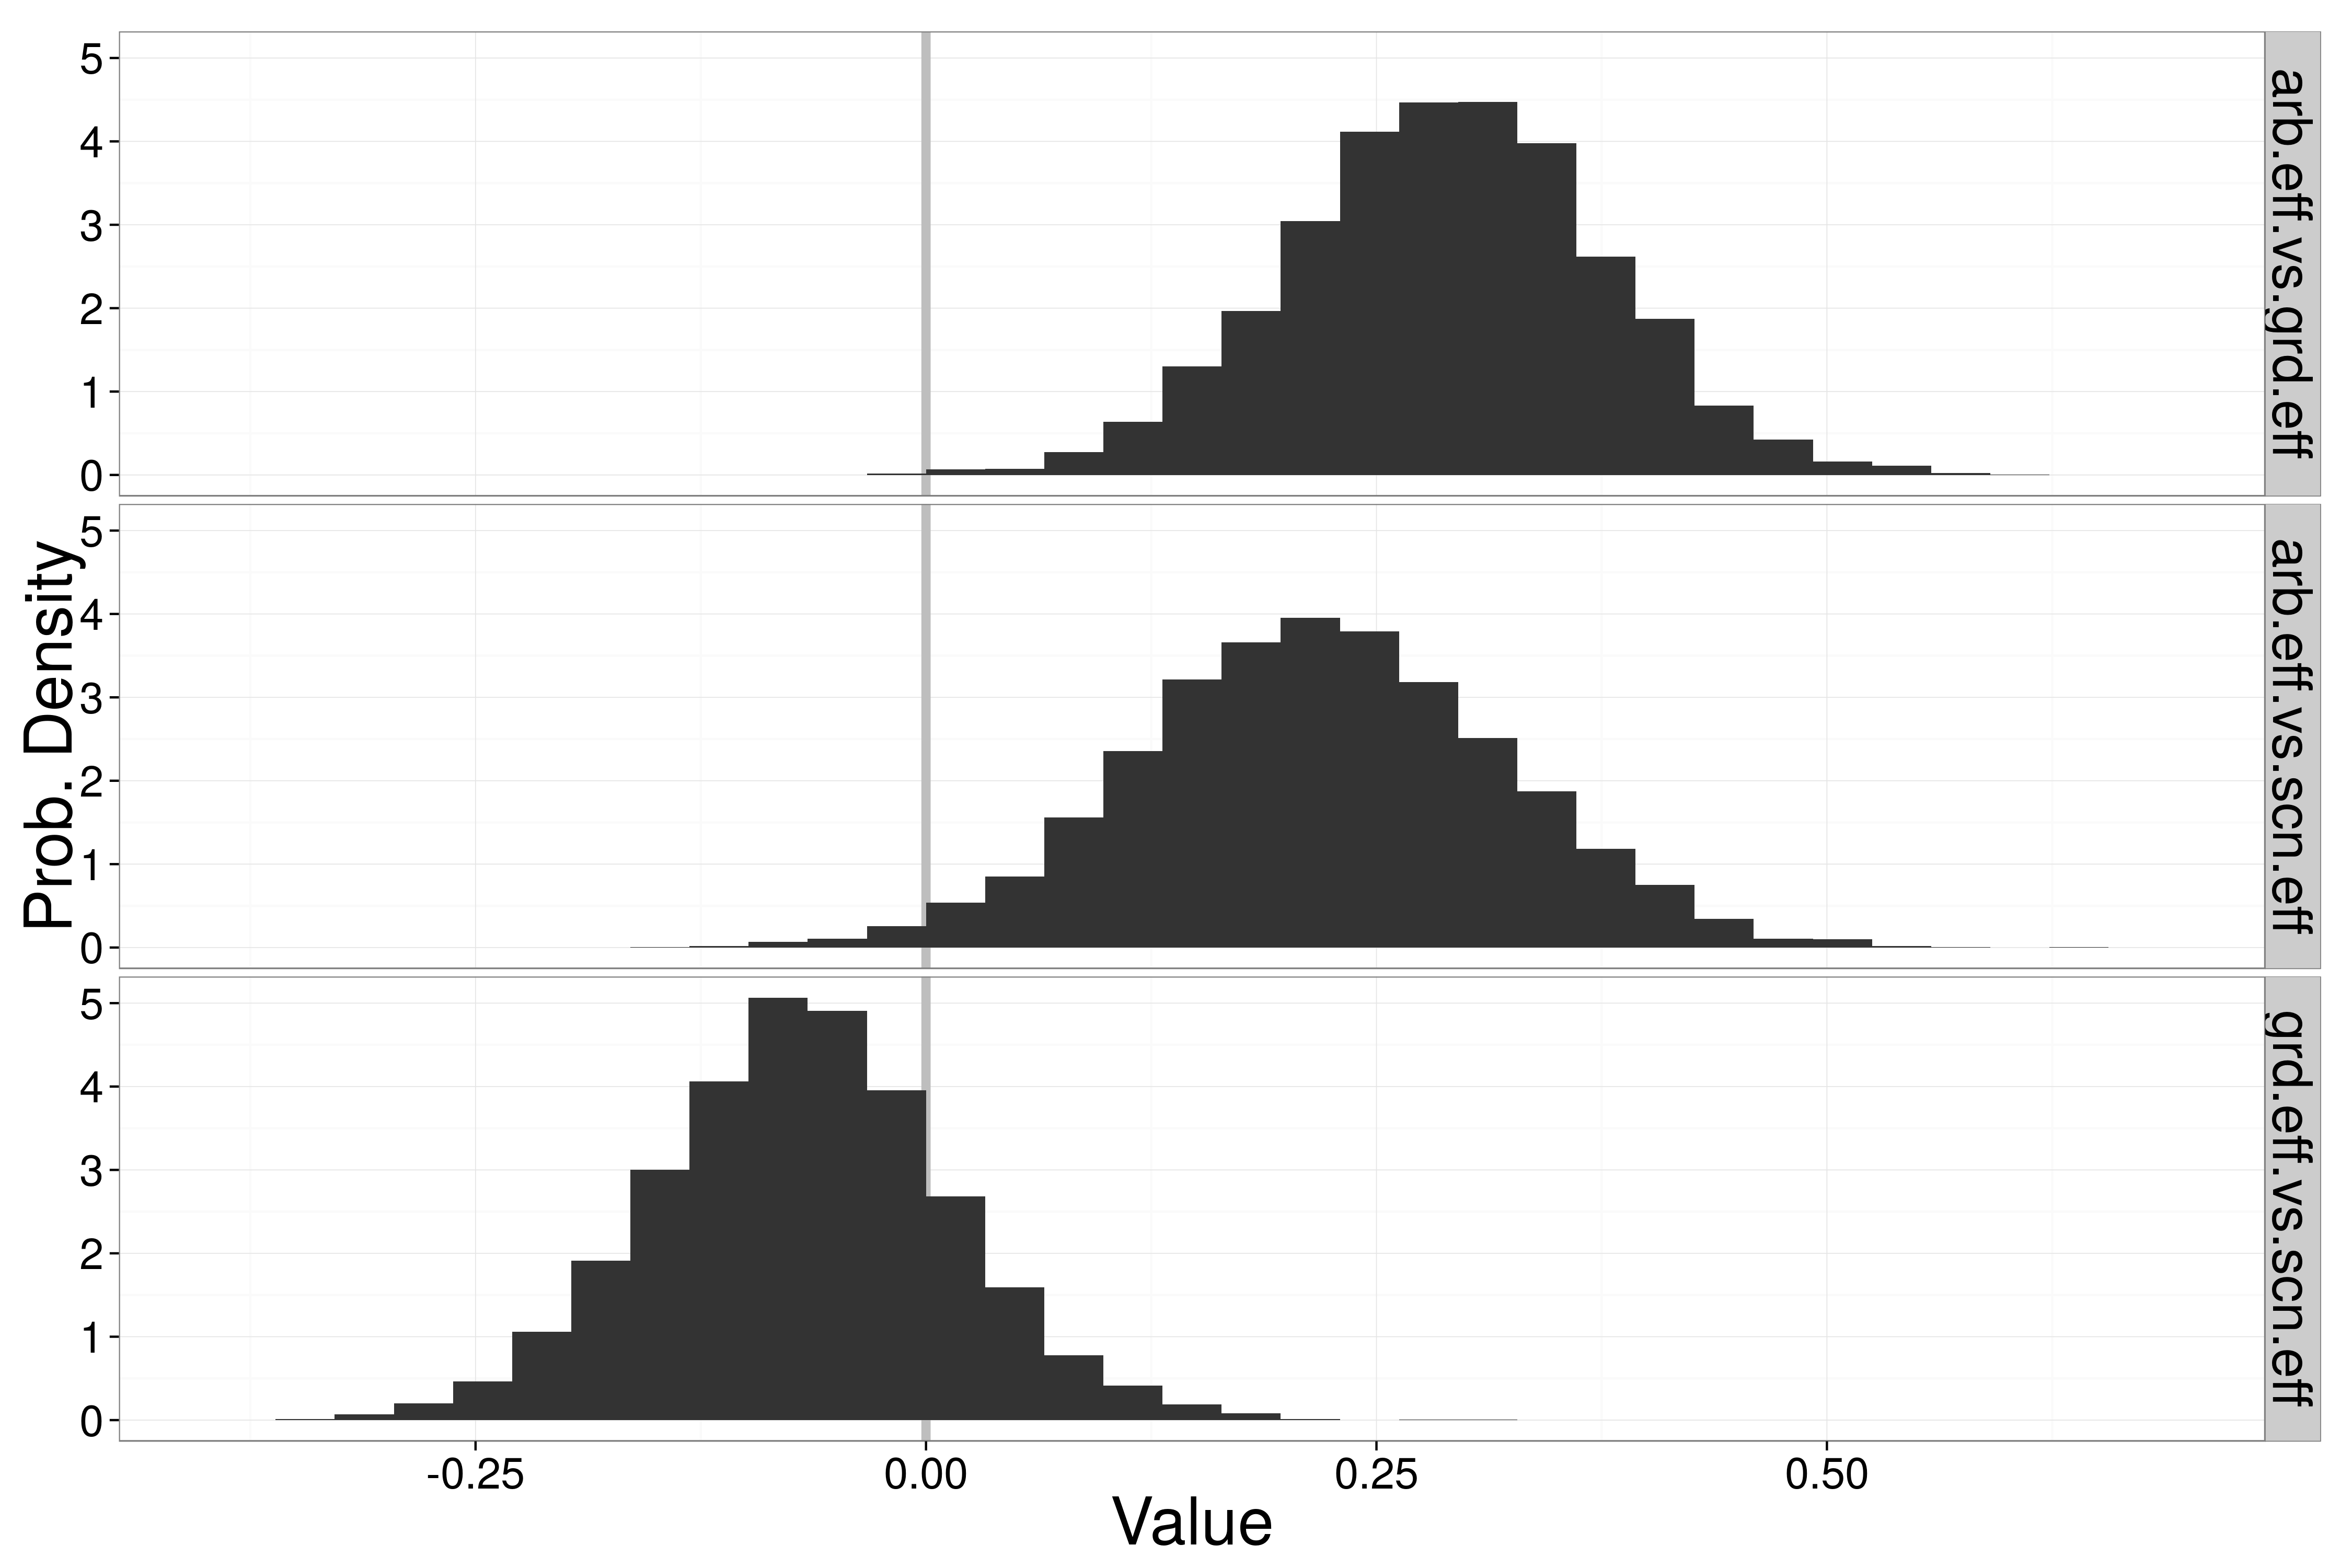
\includegraphics{figure/loco_diff_est}
    \label{subfig:loco}
  \end{subfigure}
  \begin{subfigure}[b]{0.4\textwidth}
    \caption{}
    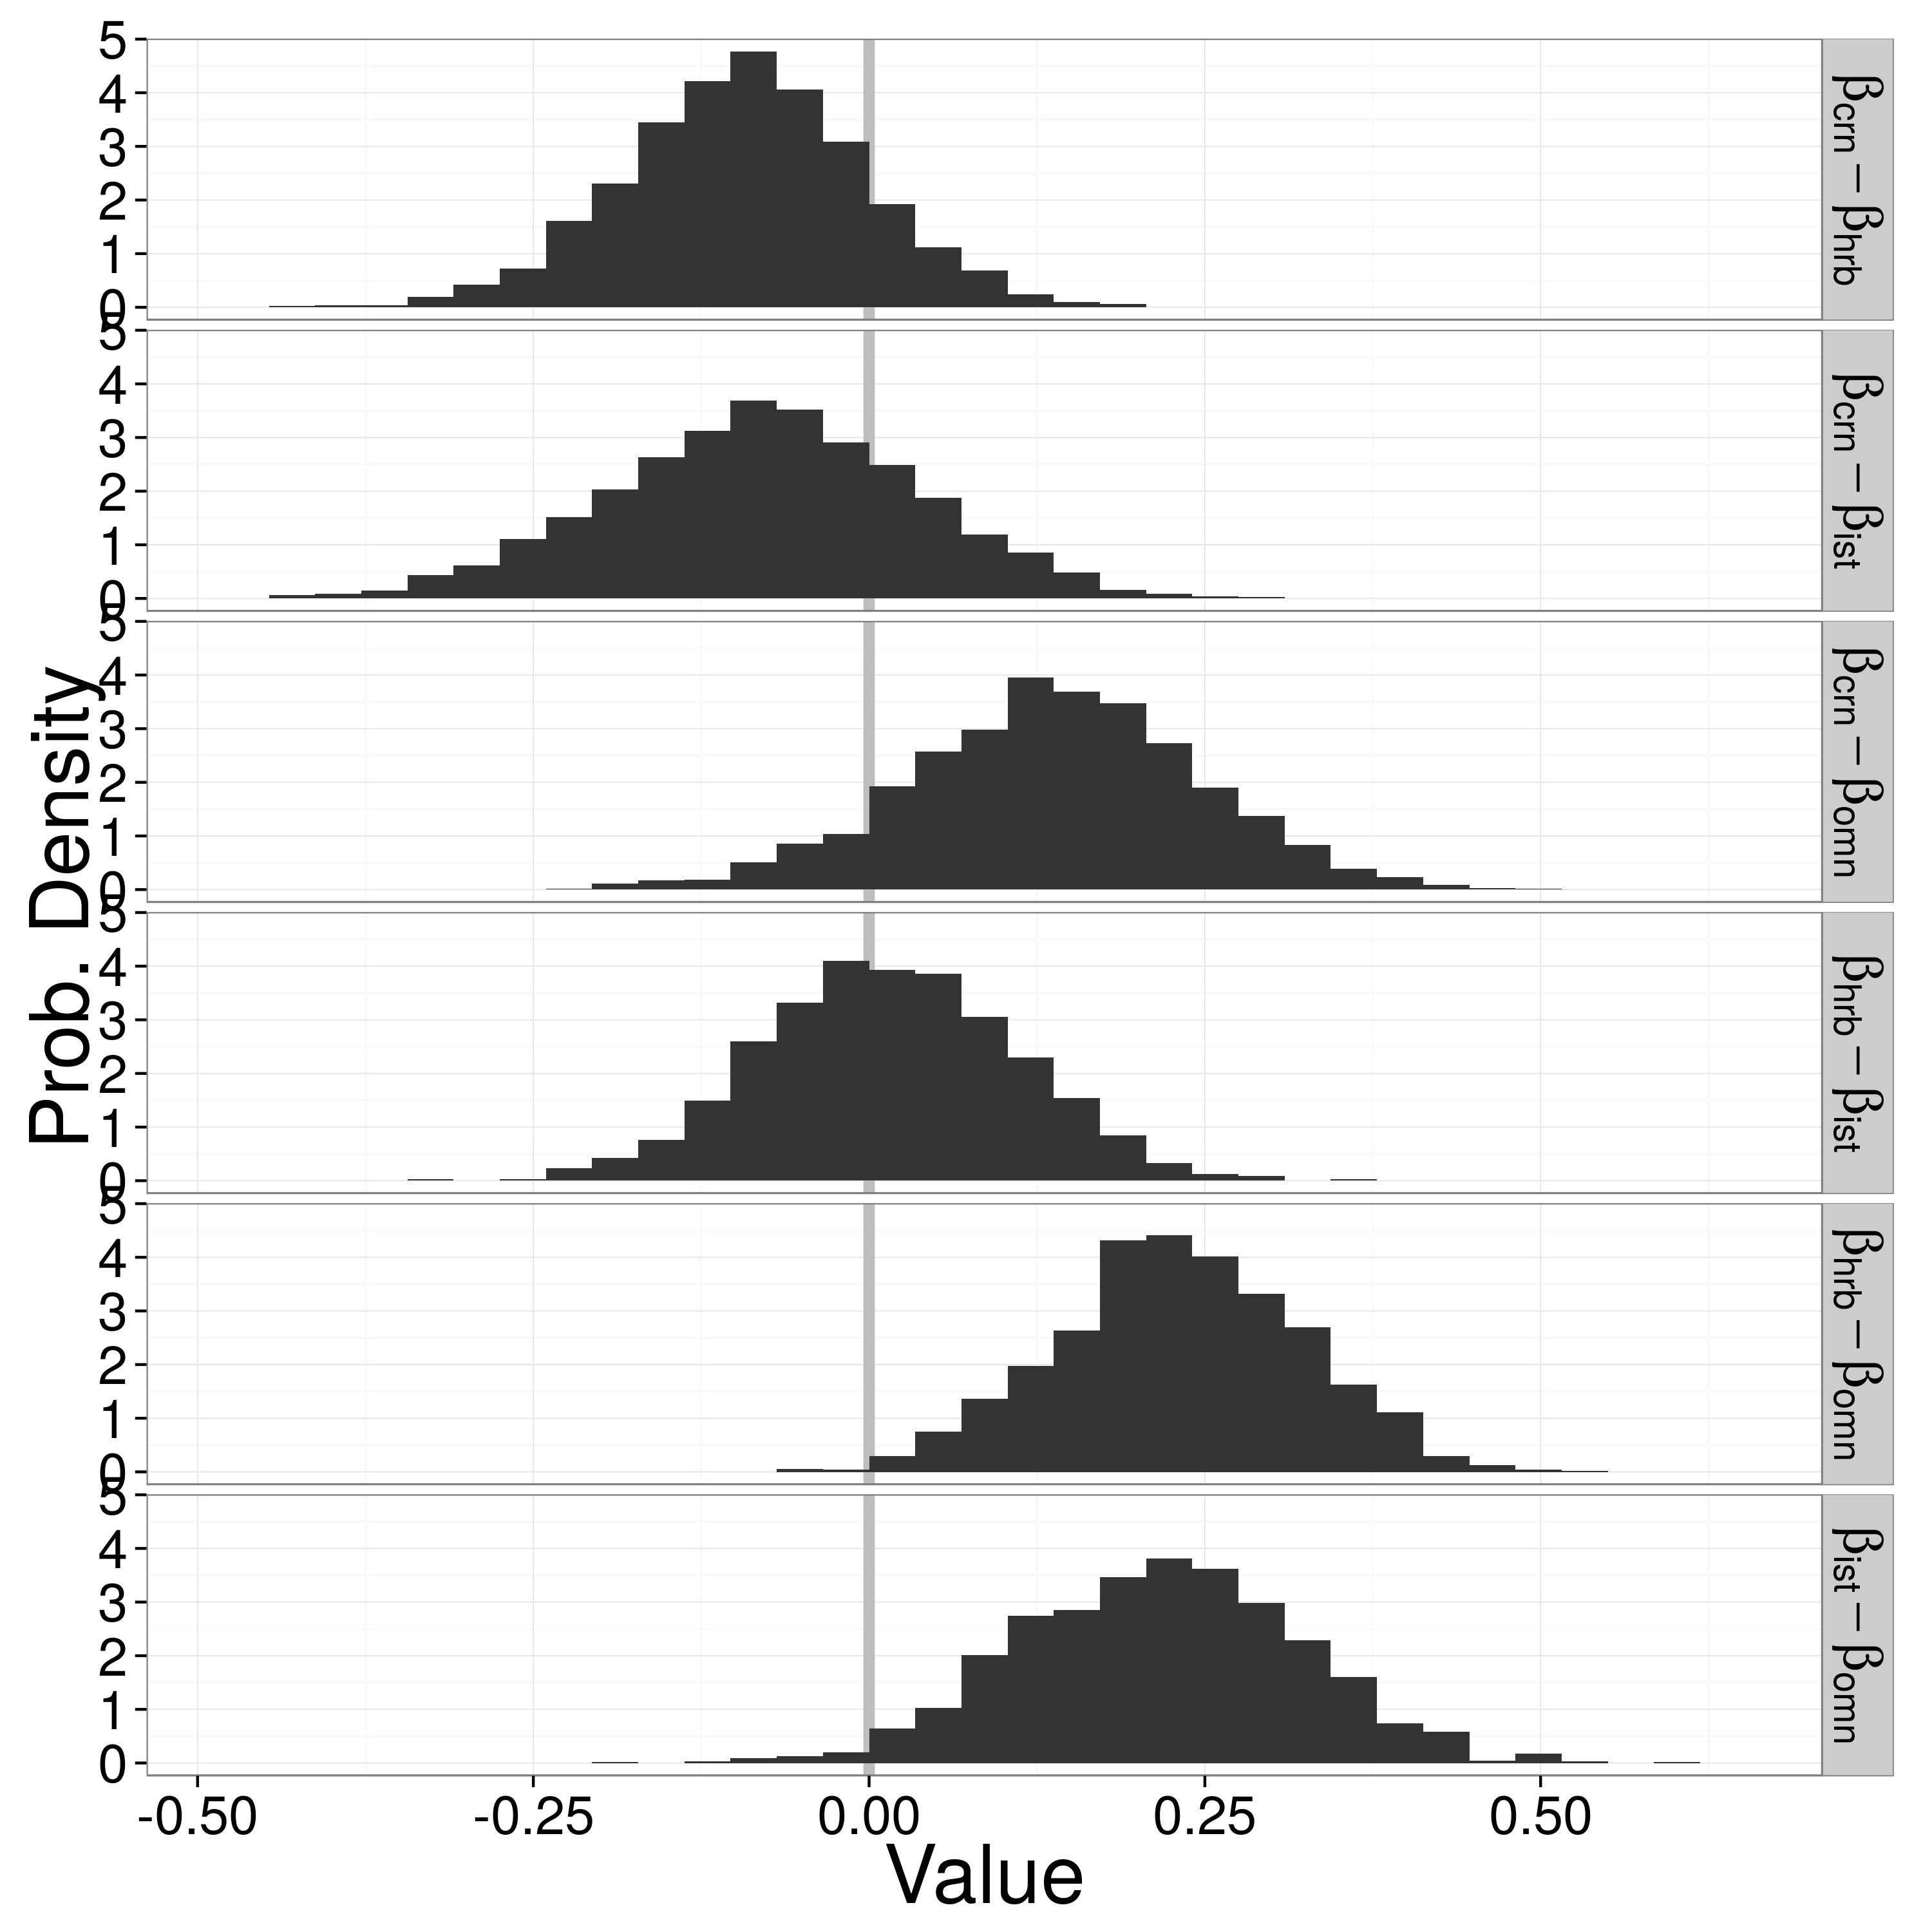
\includegraphics{figure/diet_diff_est}
    \label{subfig:diet}
  \end{subfigure}
  \caption{Pairwise differences in effect of the locomotor (\textbf{A}) and dietary categories (\textbf{B}) on expected duration from 1000 samples from the posterior distribution. Comparisons of locomotor categories, from top to bottom (\textbf{A}), are: arboreal versus ground dwelling, arboreal versus scansorial, and ground dwelling versus scansorial. For dietary category, from top to bottom (\textbf{B}): carnivore versus herbivore, carnivore versus insectivore, carnivore versus omnivore, herbivore versus insectivore, herbivore versus omnivore, and insectivore versus omnivore. Values to the left indicate that the first category is expected to have a greater duration than the second, while values to the right indicate that the first category is expected to have a shorter duration.}
  \label{fig:trait_est}
\end{figure}

\begin{figure}[ht]
  \centering
  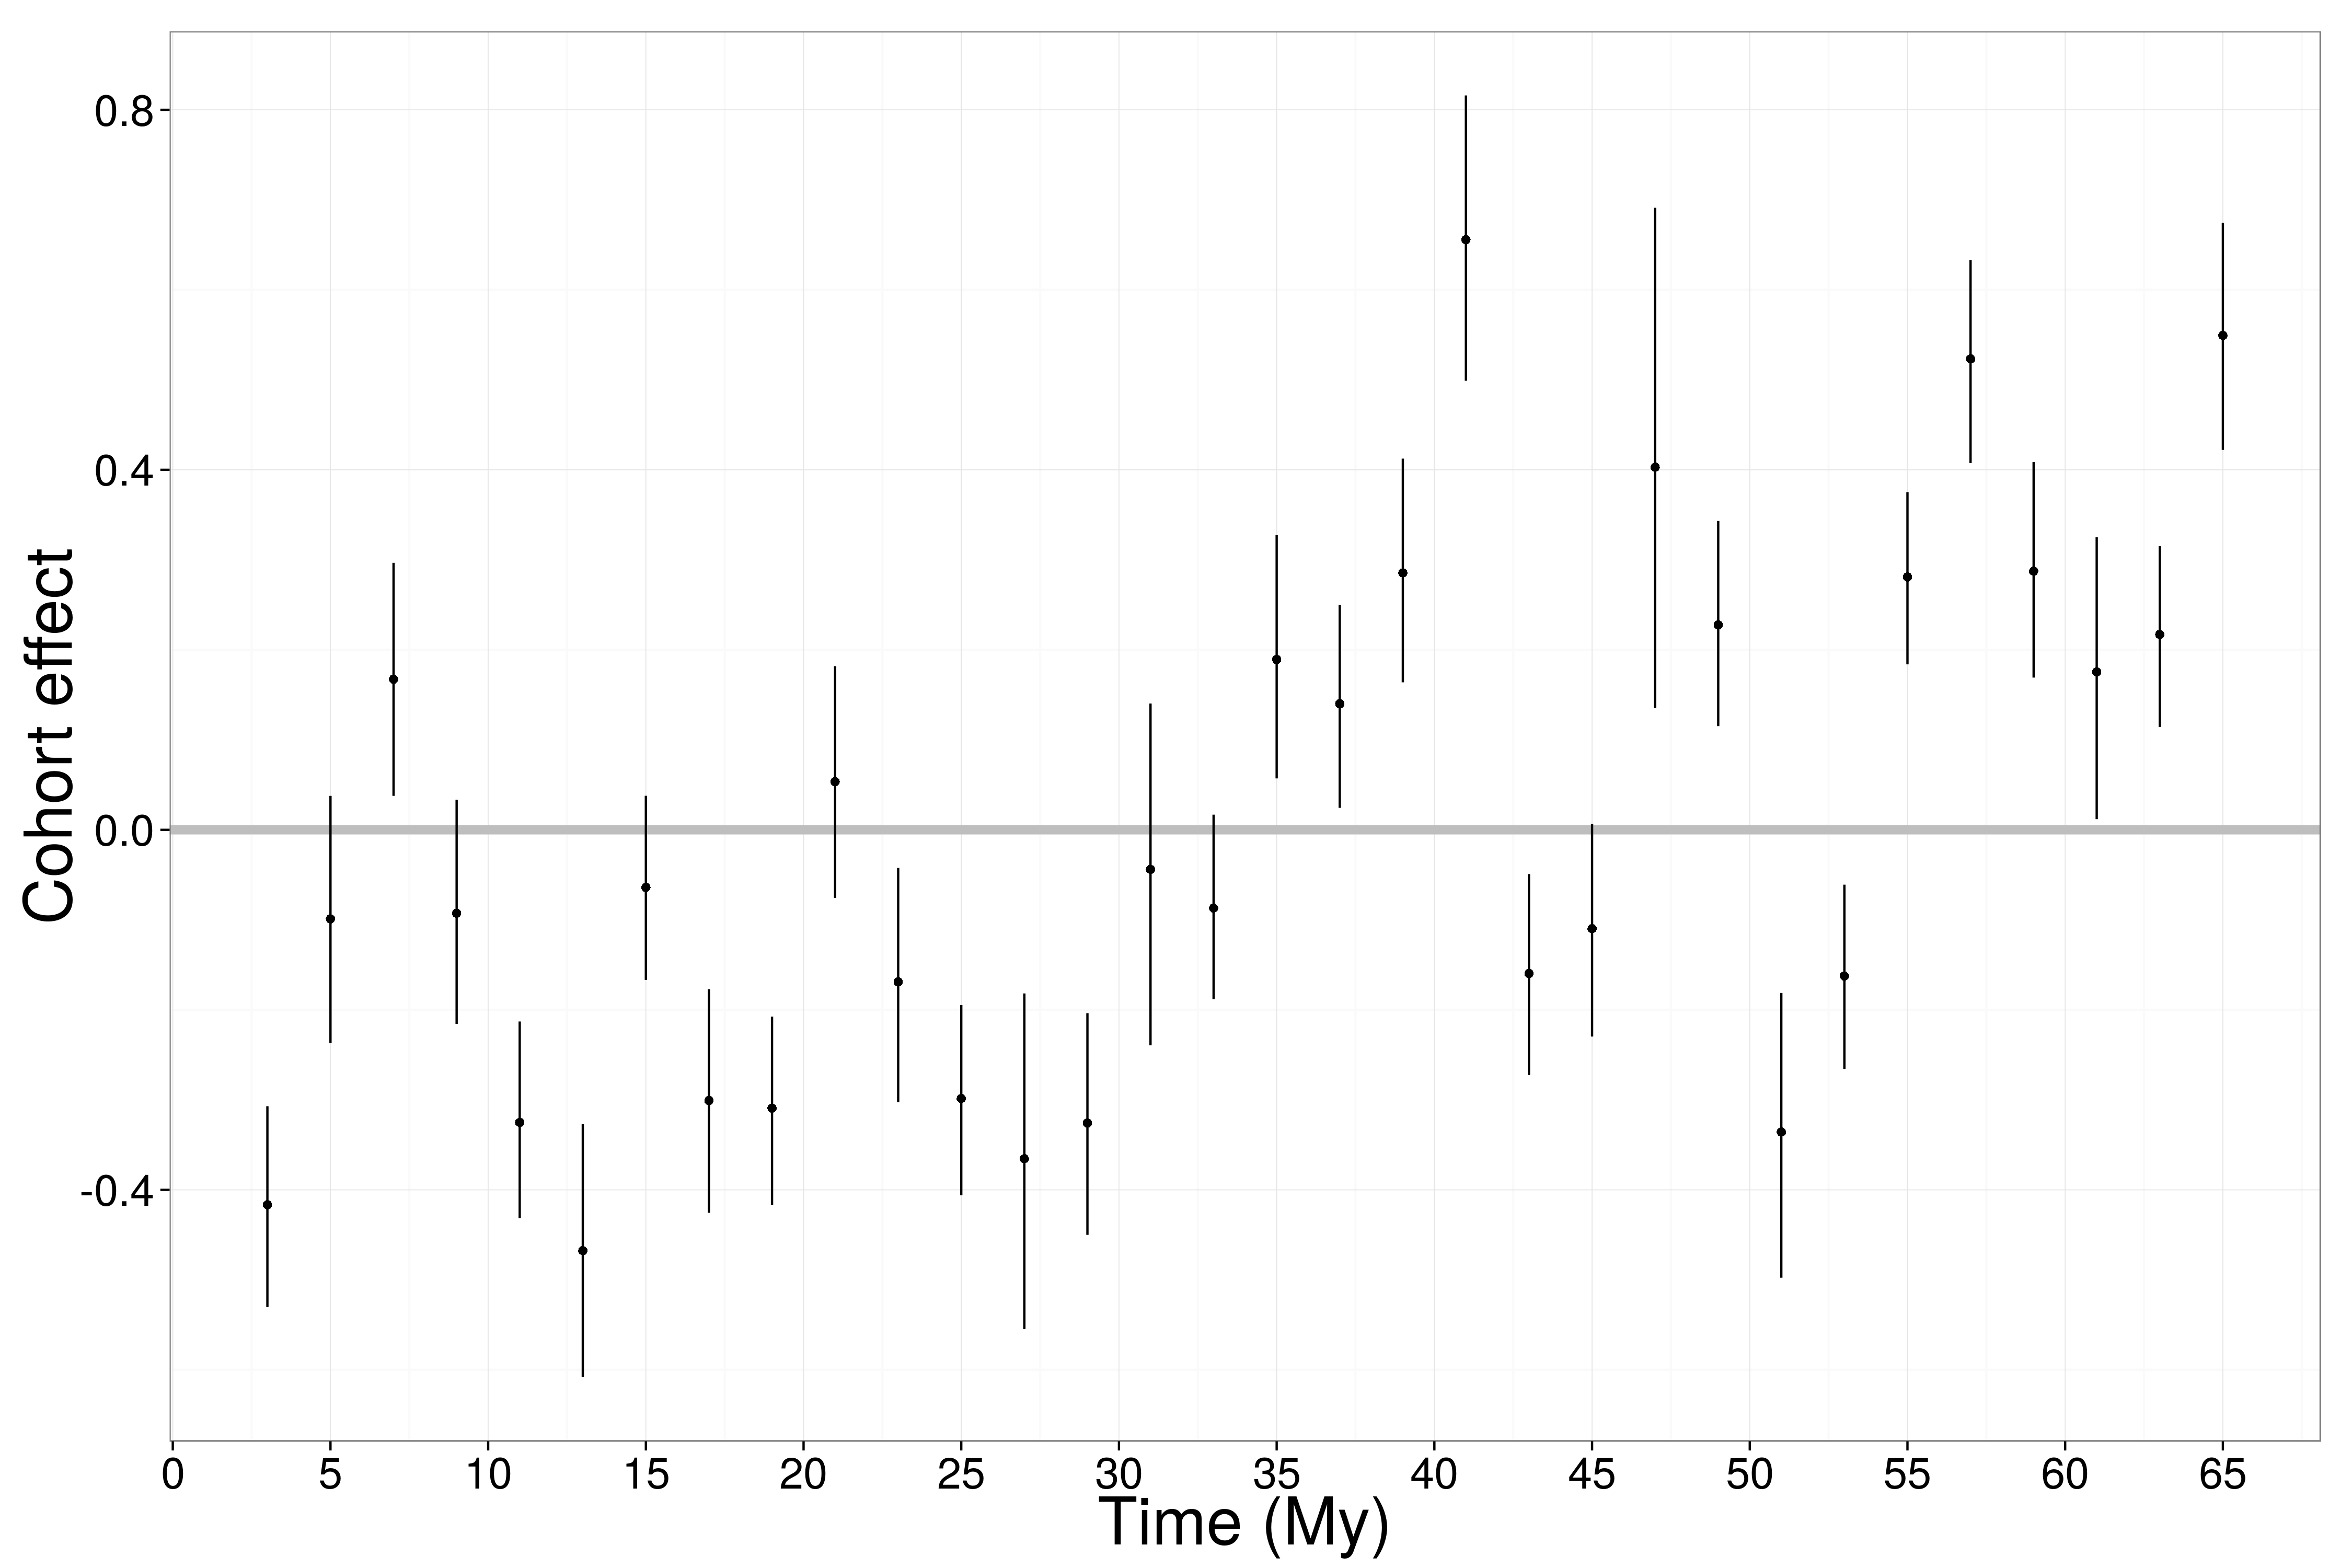
\includegraphics{figure/cohort_est}
  \caption{Summaries of posterior estimates of individual cohort effect depicted as medians and 80\% credible intervals. High values correspond to shorter species durations while lower values correspond to greater species durations compared to the mean duration. Lines are placed at the middle of the 2 My origination cohorts.}
  \label{fig:eff_cohort}
\end{figure}

\begin{figure}[ht]
  \centering
  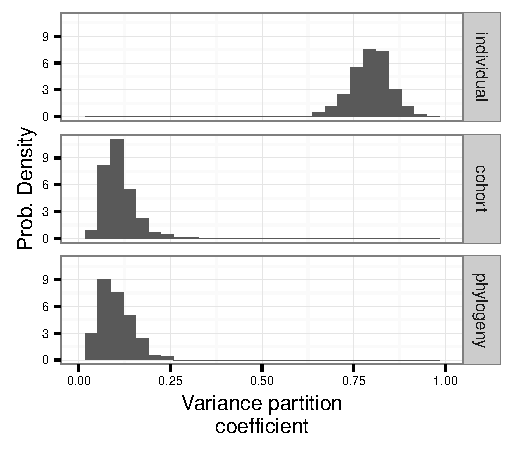
\includegraphics{figure/variance_est}
  \caption{Estimates of the variance partitioning coefficients for the three different sources of variance: species, cohort, and phylogeny. Higher values correspond to greater contribution to total observed variance. Each of the estimates is a distribution of 1000 approximating simulations due to the model's non-normally distributed errors.}
  \label{fig:vpc}
\end{figure}

% latex table generated in R 3.1.2 by xtable 1.7-4 package
% Thu Jan  8 17:45:30 2015
\begin{table}[c]
  \centering
  \begin{tabular}{rrrrrrrrr}
    & mean & sd & 2.5\% & 25\% & 50\% & 75\% & 97.5\% & \(\hat{R}\) \\ 
    \hline
    alpha & 1.29 & 0.03 & 1.23 & 1.27 & 1.29 & 1.31 & 1.36 & 1.00 \\ 
    intercept & -0.78 & 0.14 & -1.05 & -0.87 & -0.78 & -0.68 & -0.51 & 1.00 \\ 
    logit(occupancy) & -0.53 & 0.08 & -0.69 & -0.59 & -0.53 & -0.48 & -0.38 & 1.00 \\ 
    log(size) & -0.05 & 0.05 & -0.14 & -0.08 & -0.05 & -0.01 & 0.05 & 1.00 \\ 
    ground dwelling & -0.28 & 0.10 & -0.47 & -0.34 & -0.28 & -0.21 & -0.09 & 1.00 \\ 
    scansorial & -0.22 & 0.11 & -0.43 & -0.29 & -0.22 & -0.14 & -0.00 & 1.00 \\ 
    herbivore & 0.09 & 0.09 & -0.09 & 0.03 & 0.09 & 0.14 & 0.27 & 1.00 \\ 
    insectivore & 0.10 & 0.11 & -0.11 & 0.03 & 0.10 & 0.17 & 0.31 & 1.00 \\ 
    omnivore & -0.12 & 0.11 & -0.33 & -0.19 & -0.12 & -0.05 & 0.09 & 1.00 \\ 
    \hline
    sd cohort & 0.33 & 0.06 & 0.23 & 0.29 & 0.33 & 0.37 & 0.48 & 1.00 \\ 
    sd phylogeny & 0.11 & 0.05 & 0.03 & 0.07 & 0.10 & 0.14 & 0.23 & 1.03 \\ 
    \hline
  \end{tabular}
  \caption{Marginal posterior estimates for the praameters of interested based on 1000 posterior samples. The intercept can be interpreted as the estimate for the mean observed species. The other values are the effect of a trait on the expected species duration as expressed as deviation from the mean. The categorical variables are binary index variables where an observation is of that category or not. \(\hat{R}\) values of less than 1.1 indicate approximate chain convergence for the posterior samples.}
  \label{tab:post_sum}
\end{table}



\end{document}


